\documentclass{beamer}
\usepackage{amsmath, amssymb}
\usepackage{physics}
\usepackage{subfig}
\usepackage{hyperref}

\usepackage[utf8]{inputenc}
\usetheme{Madrid}

\title{Usage of JEWEL generator}
\author{Jinghong Yang}

\AtBeginSection[]
{
  \begin{frame}
    \frametitle{Table of Contents}
    \tableofcontents[currentsection]
  \end{frame}
}

\begin{document}

\begin{frame}
\titlepage
\end{frame}

\begin{frame}
\frametitle{Table of Contents}
\tableofcontents
\end{frame}

\section{Installation}
\begin{frame}
 \frametitle{Installing prerequisites}

 \begin{figure}[h]
  \centering
  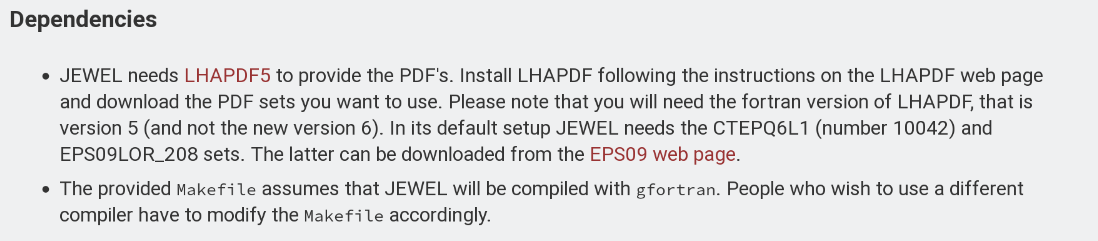
\includegraphics[width=0.9\linewidth]{dependencies.png}
 \end{figure}

 \begin{block}{Download and Install LHAPDF5}
 \begin{scriptsize}
  \url{https://lhapdf.hepforge.org/downloads?f=old}
  \url{https://lhapdf.hepforge.org/lhapdf5/install}
  \end{scriptsize}
 \end{block}

 \begin{block}{\href{https://lhapdf.hepforge.org/lhapdf5/manual\#tth_sEcA}{Download PDF sets (e.g. 5.9.1)} }
 \begin{scriptsize}
  \url{https://lhapdf.hepforge.org/downloads/?f=pdfsets/5.9.1/EPS09LOR_208.LHgrid}
  \url{https://lhapdf.hepforge.org/downloads?f=pdfsets/5.9.1//cteq6ll.LHpdf}\\
\end{scriptsize}
\begin{footnotesize}
Put them in (lhapdf path)\textit{/share/lhapdf/PDFsets/}
\end{footnotesize}
\end{block}

\begin{tiny}
\href{https://www.jyu.fi/science/en/physics/research/highenergy/urhic/npdfs/eps09}{alternative}
\end{tiny}


\end{frame}

\begin{frame}
 \frametitle{Compiling JEWEL}
 \begin{block}{Modify Makefile}
 LHAPDF\_PATH := (your lhapdf install path)/lib/
 \end{block}

 \begin{block}{Modifying your .bashrc or .zshrc}
 export LD\_LIBRARY\_PATH=/.../lhapdf-5.x.y/lib:\$LD\_LIBRARY\_PATH
 export LHAPATH=/.../lhapdf-5.x.y/share/lhapdf/PDFsets
 \end{block}
\end{frame}


\section{Data generation}
\begin{frame}
\frametitle{Run JEWEL}
\begin{itemize}
 \item Now you have two binaries: jewel-2.2.0-vac and jewel-2.2.0-simple
 \item ./jewel-2.2.0-vac $\langle$configuration file$\rangle$
 \item ./jewel-2.2.0-simple $\langle$configuration file$\rangle$
 \item \href{https://arxiv.org/pdf/1311.0048.pdf}{Documentation}
\end{itemize}

\begin{alertblock}{Caution}
Watch out for xsecs.dat, pdf.dat, and splitint.

If you change physical parameters, delete these files before you run JEWEL again.
\end{alertblock}



\end{frame}

\section{Generate gluon and quark jets}

\begin{frame}
 \begin{itemize}
  \item Show routine initpythia in jewel-2.2.0.f (roughly line 800)
  \item \href{https://pythia.org/download/pythia6/lutp0613man2.pdf}{Pythia 6 Documentation} (See pages 140, 145, and 195)
 \end{itemize}

%  \begin{co

\end{frame}


\section{Data processing using RIVET}

\begin{frame}
 \frametitle{RIVET installation}
 % mention apptainer vs native install vs docker
\end{frame}

\begin{frame}
 \frametitle{Using apptainer or docker}
\end{frame}

% if have time, talk a little bit more about native install

% mention jewel mkfifo
\begin{frame}
 \frametitle{Using named pipe}
\end{frame}


\section{Troubleshooting}

\end{document}


